\documentclass[a4paper, 12pt]{article}
\usepackage[top=2cm, bottom=2cm, left=2.5cm, right=2.5cm]{geometry}
\usepackage[utf8]{inputenc}
\usepackage{array}
\usepackage{graphicx}
\usepackage{listings}
\usepackage{caption}
\usepackage{float}
\usepackage[labelfont=bf]{caption}
\captionsetup[lstlistings]{position=bottom}
\graphicspath{{img/}}
\lstset{language=SQL}
\begin{document}
\noident
\textbf{UNIVERSIDADE TECNOLÓGICA FEDERAL DO PARANÁ | UTFPR}
\textbf{ALUNO:} Ricardo Medeiros da Costa Junior   \textbf{RA:} a1598996 \\
\textbf{DISCIPLINA:} Programação para Bioinformática \\
\textbf{ATIVIDADE:} Lista de Exercícios 1  

\section{Para cada exercício faça}
\begin{enumerate}
\item Análise do Problema
\item Algoritmo
\item Fluxograma
\item Teste de mesa
\end{enumerate}

\begin{enumerate}
  \item Dado dois números naturais verificar quem é o maior
    \begin{description}
      
    \end{description}
  \item Dado dois números naturais verificar quem é o maior
    \begin{description}
      \item[Análise do Problema:] O exercício pede que dado dois números naturais deve-se verificar qual é o maior.
Um procedimento razoável para resolver esse problema é verificar se as entradas são válidas (se são números naturais) e assim informar qual é o maior ou se não houver maior, que os números são iguais. 

      \item[Algoritmo:]
         \begin{figure}[H]
         \centering
         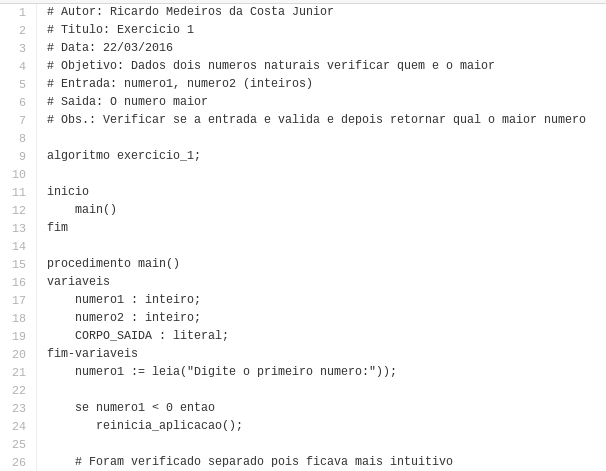
\includegraphics[width=1\textwidth]{ex1_1}
         \caption[Algoritmo Exercício 1]{\textbf{Algoritmo 1}}
         \end{figure}
         \begin{figure}[H]
         \centering
         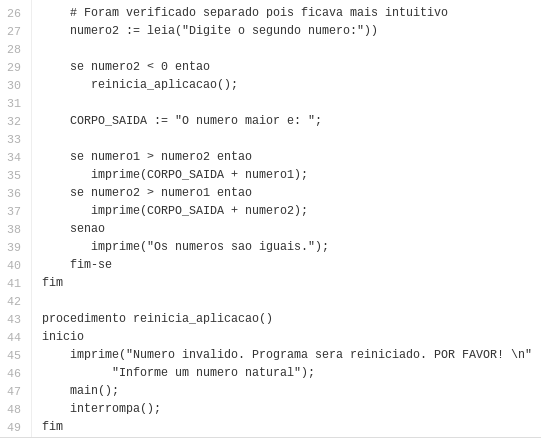
\includegraphics[width=1\textwidth]{ex1_2}
         \caption[Algoritmo Exercício 1]{\textbf{Algoritmo 1}}
         \end{figure} 
         

      \item[Fluxograma:]
         \begin{figure}[H]
         \centering
         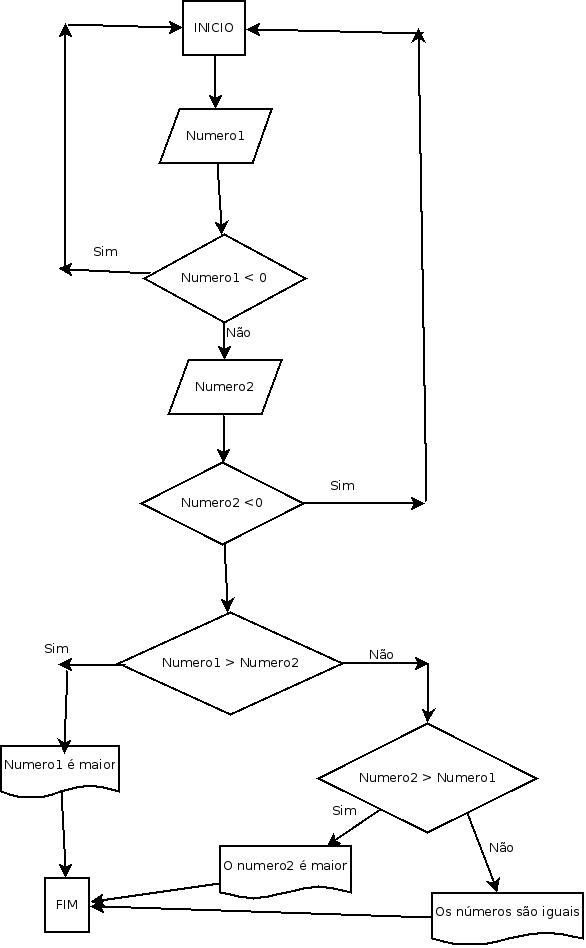
\includegraphics[width=1\textwidth]{fluxograma1}
         \caption[Fluxograma 1]{\textbf{Fluxograma 1}}
         \end{figure}
         
       \item[Teste de mesa:]
         \begin{figure}[H]
         \centering
         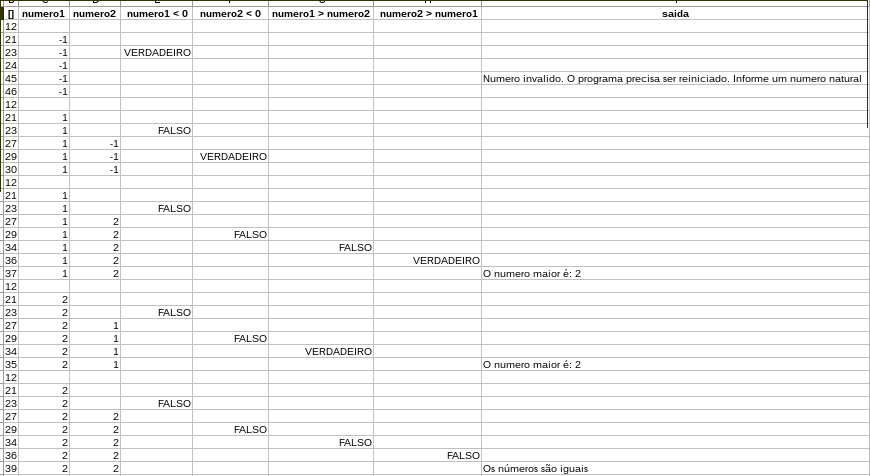
\includegraphics[width=1\textwidth]{teste1}
         \caption[Teste de mesa 1]{\textbf{Teste de mesa 1}}
         \end{figure}          
    \end{description}
  \item Dado 4 notas, calcular a média aritmética.
    \begin{description}
      \item[Análise do Problema:] O exercício pede que seja informado a média aritmética de 4 notas informadas pelo usuário. Uma abordagem é solicitar que o usuário informe as 4 notas, validar se as entradas são válidas (ou seja, que são números positivos dos conjuntos dos reais), calcular a média aritmética (o somatório das notas dividido pela quantidade de notas) e informar o resultado para o usuário.

      \item[Algoritmo:]
         \begin{figure}[H]
         \centering
         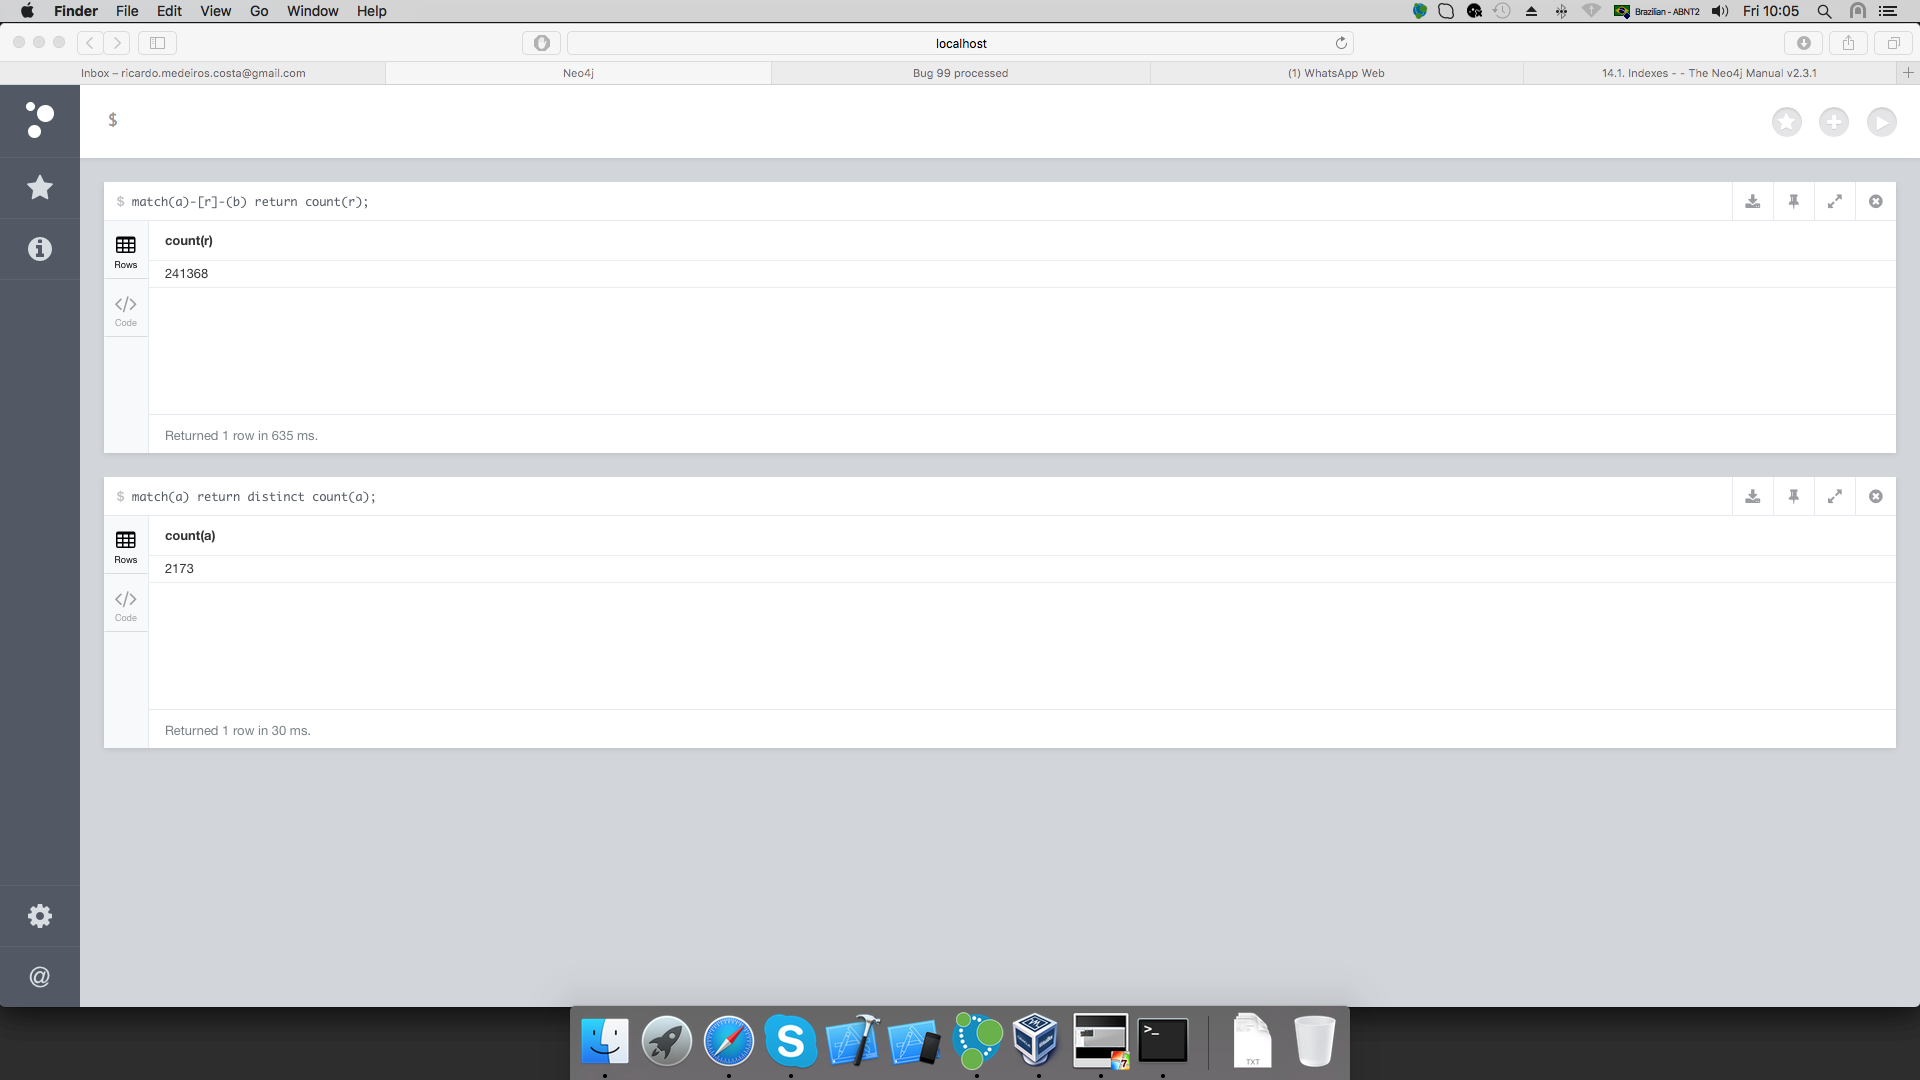
\includegraphics[width=1\textwidth]{1}
         \caption[1 - Quantidade de nós e relações]{\textbf{Quantidade de nós e relações}}
         \end{figure} 
        
       \item[Fluxograma:]
         \begin{figure}[H]
         \centering
         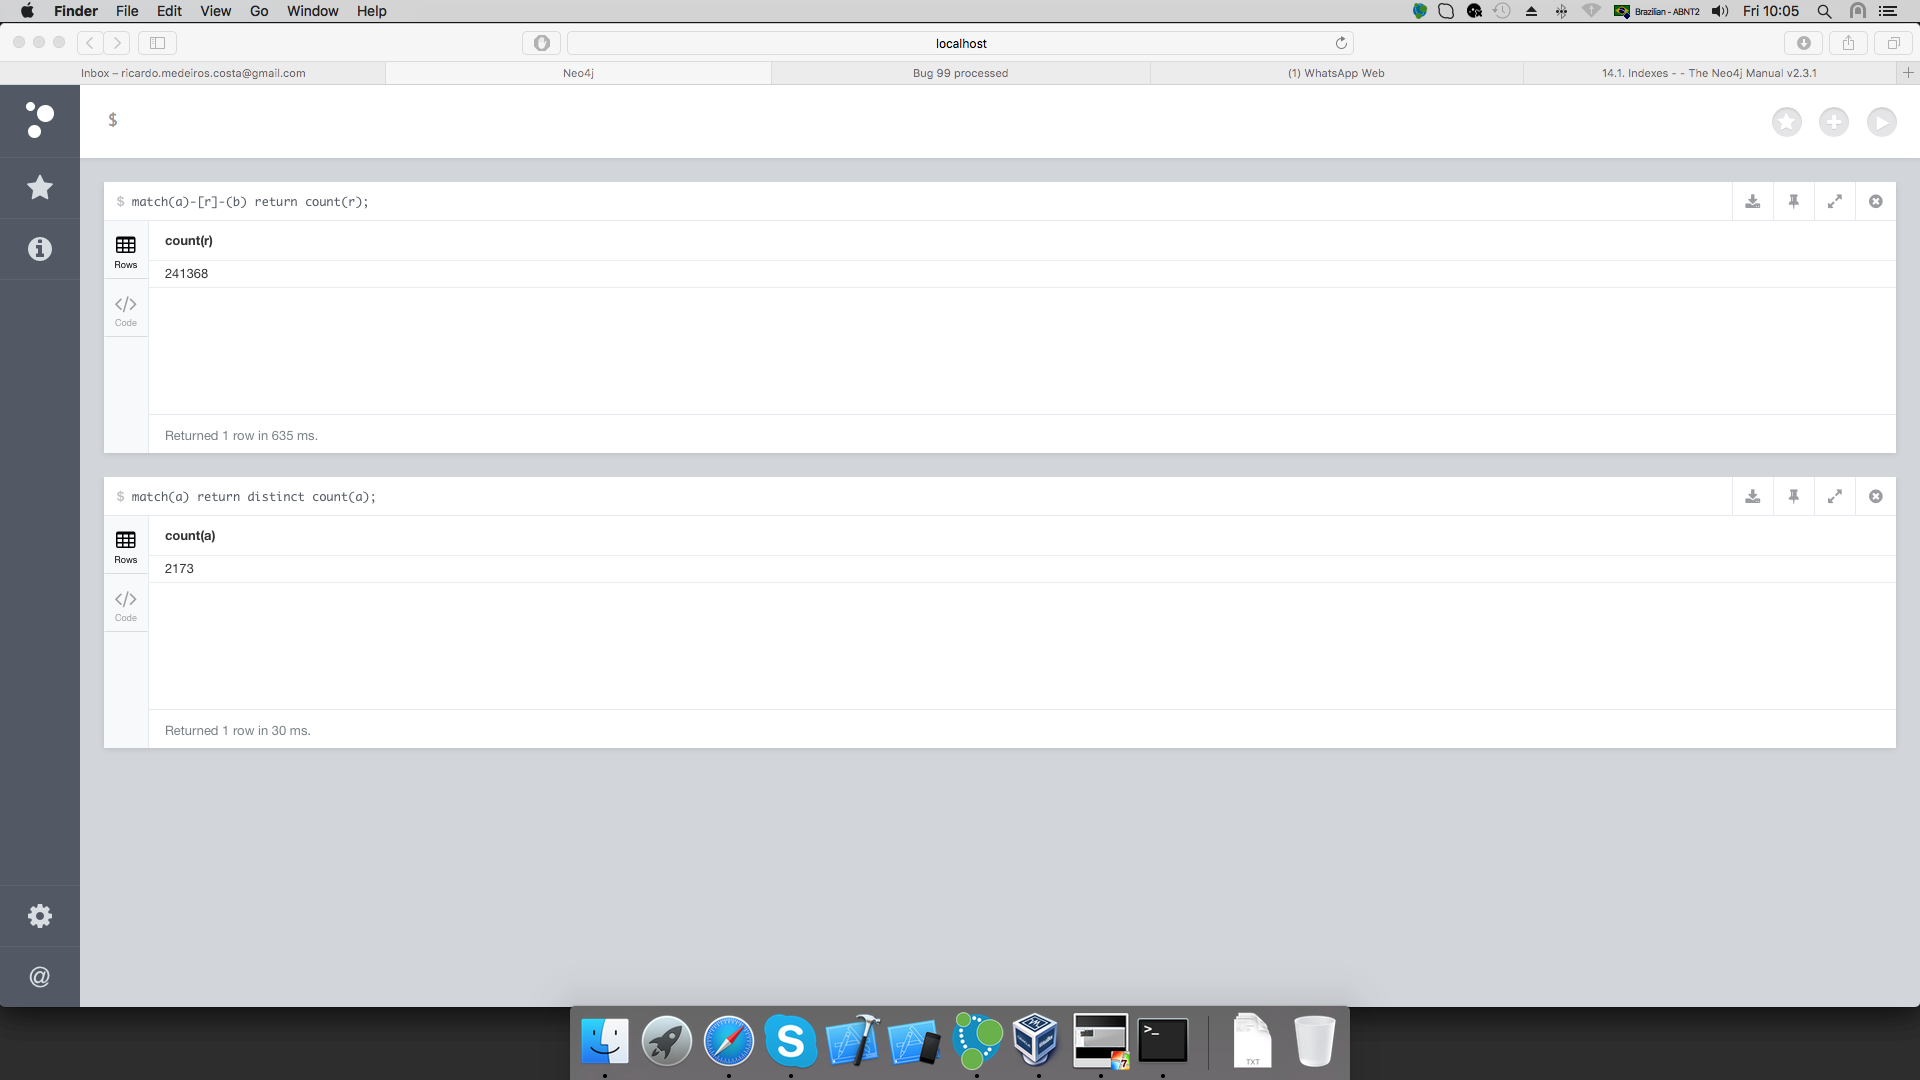
\includegraphics[width=1\textwidth]{1}
         \caption[1 - Quantidade de nós e relações]{\textbf{Quantidade de nós e relações}}
         \end{figure} 
         
       \item[Teste de mesa:]
         \begin{figure}[H]
         \centering
         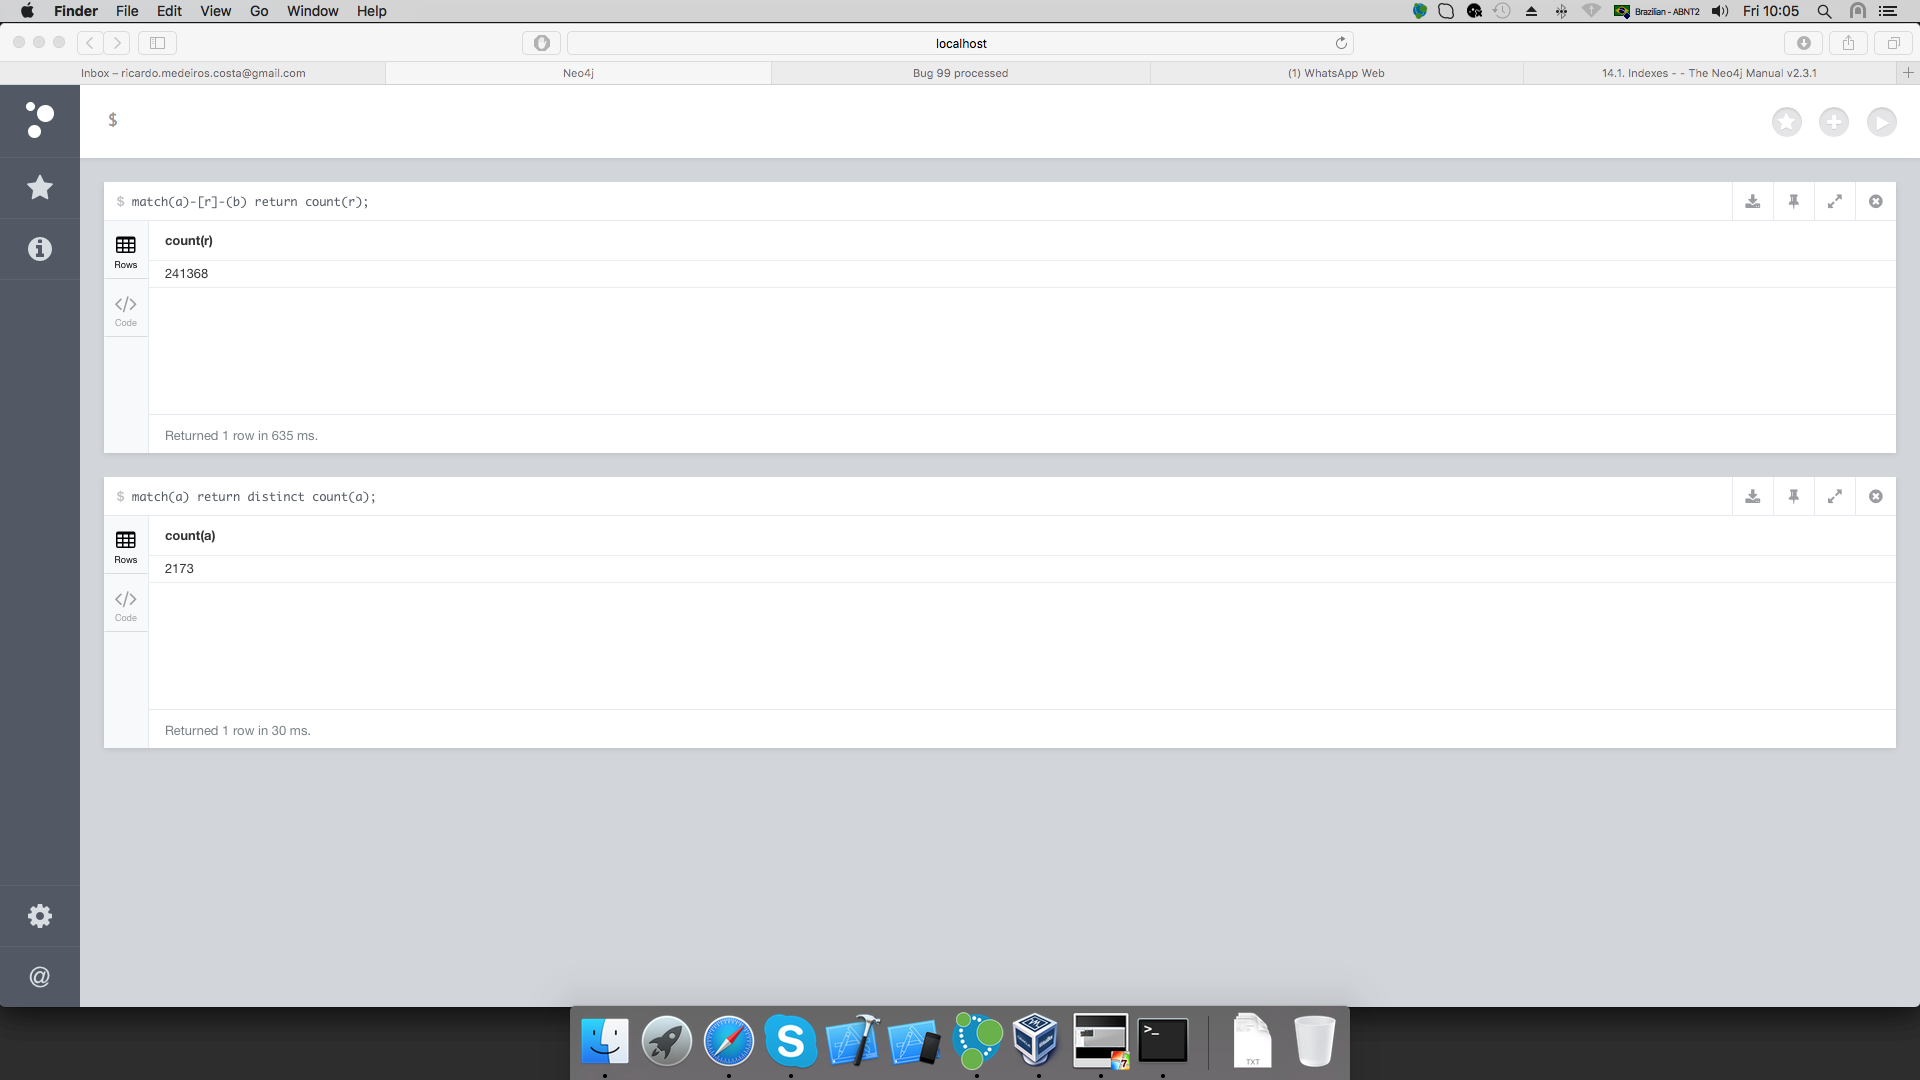
\includegraphics[width=1\textwidth]{1}
         \caption[1 - Quantidade de nós e relações]{\textbf{Quantidade de nós e relações}}
         \end{figure} 
         
    \end{description}
  \item Dado 3 notas, calcular a média ponderada sendo nota 1 peso 2, nota 2 peso 5 e nota 3 peso 3.
    \begin{description}
      \item[Análise do Problema:] O exercício pede que seja calculada a média ponderada de 3 notas, sendo a primeira nota com peso 2, a segunda com peso 5 e a terceira com peso 3. Uma solução para esse problema é solicitar que o usuário informe as 3 notas, validá-las (verificar se são números positivos pertencentes ao conjunto dos números reais), calcular a média poderada (somatório de cada nota multiplicado pelo seu peso dividido pelo somatório dos pesos) e informar o resultado ao usuário.

      \item[Algoritmo:]
         \begin{figure}[H]
         \centering
         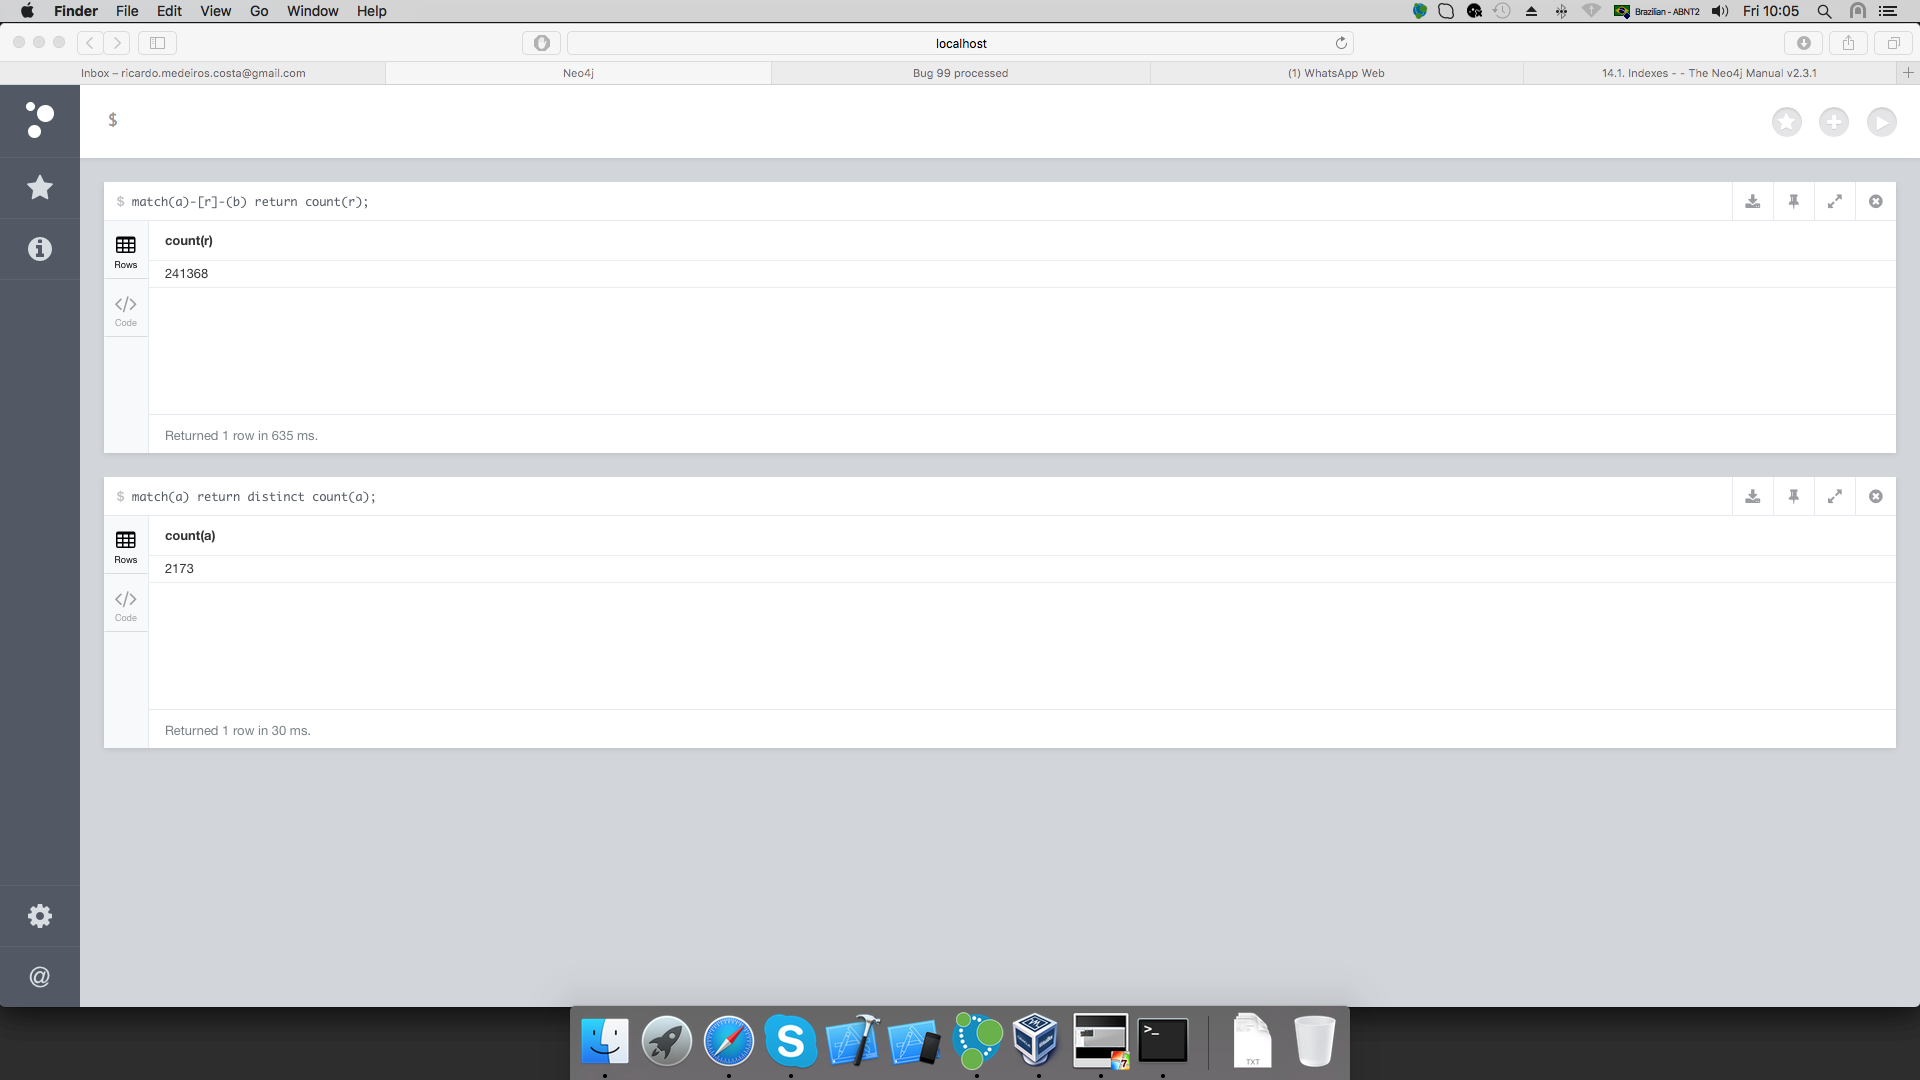
\includegraphics[width=1\textwidth]{1}
         \caption[1 - Quantidade de nós e relações]{\textbf{Quantidade de nós e relações}}
         \end{figure} 
        
       \item[Fluxograma:]
         \begin{figure}[H]
         \centering
         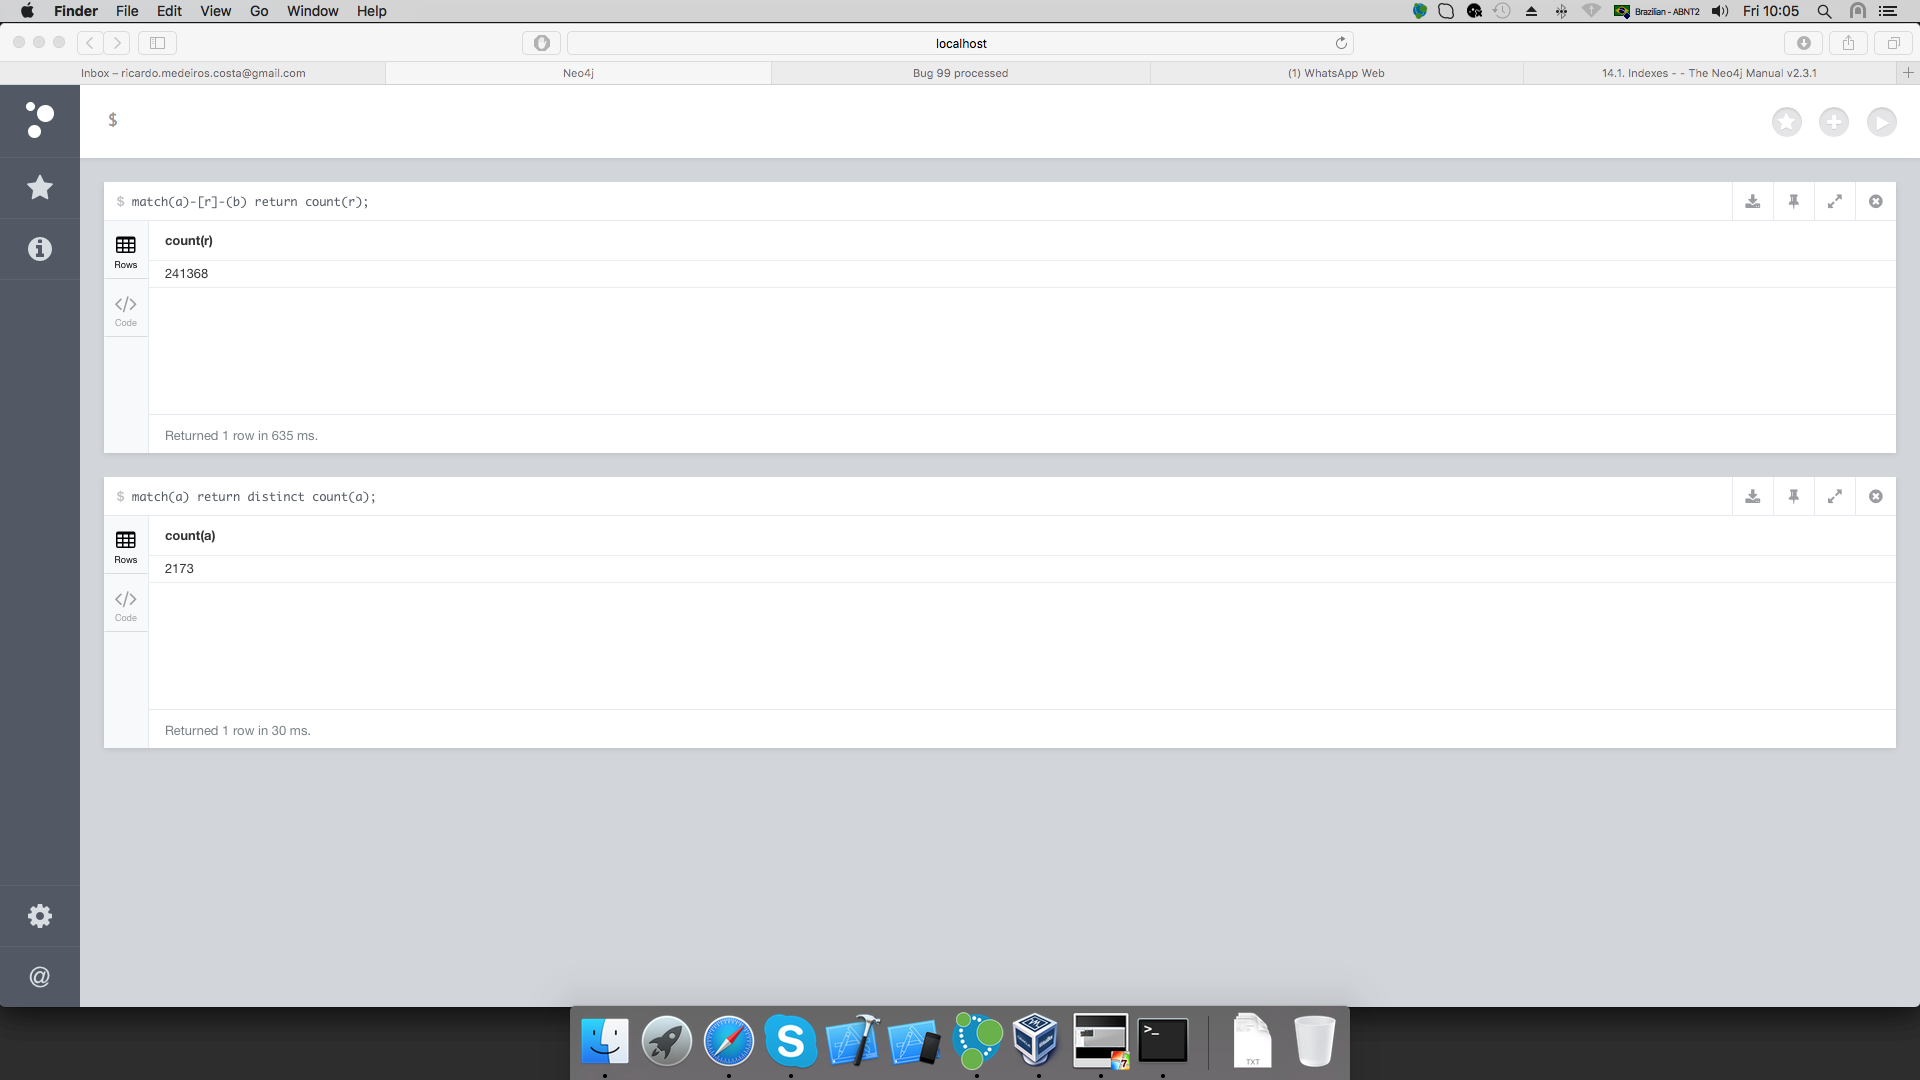
\includegraphics[width=1\textwidth]{1}
         \caption[1 - Quantidade de nós e relações]{\textbf{Quantidade de nós e relações}}
         \end{figure} 
         
       \item[Teste de mesa:]
         \begin{figure}[H]
         \centering
         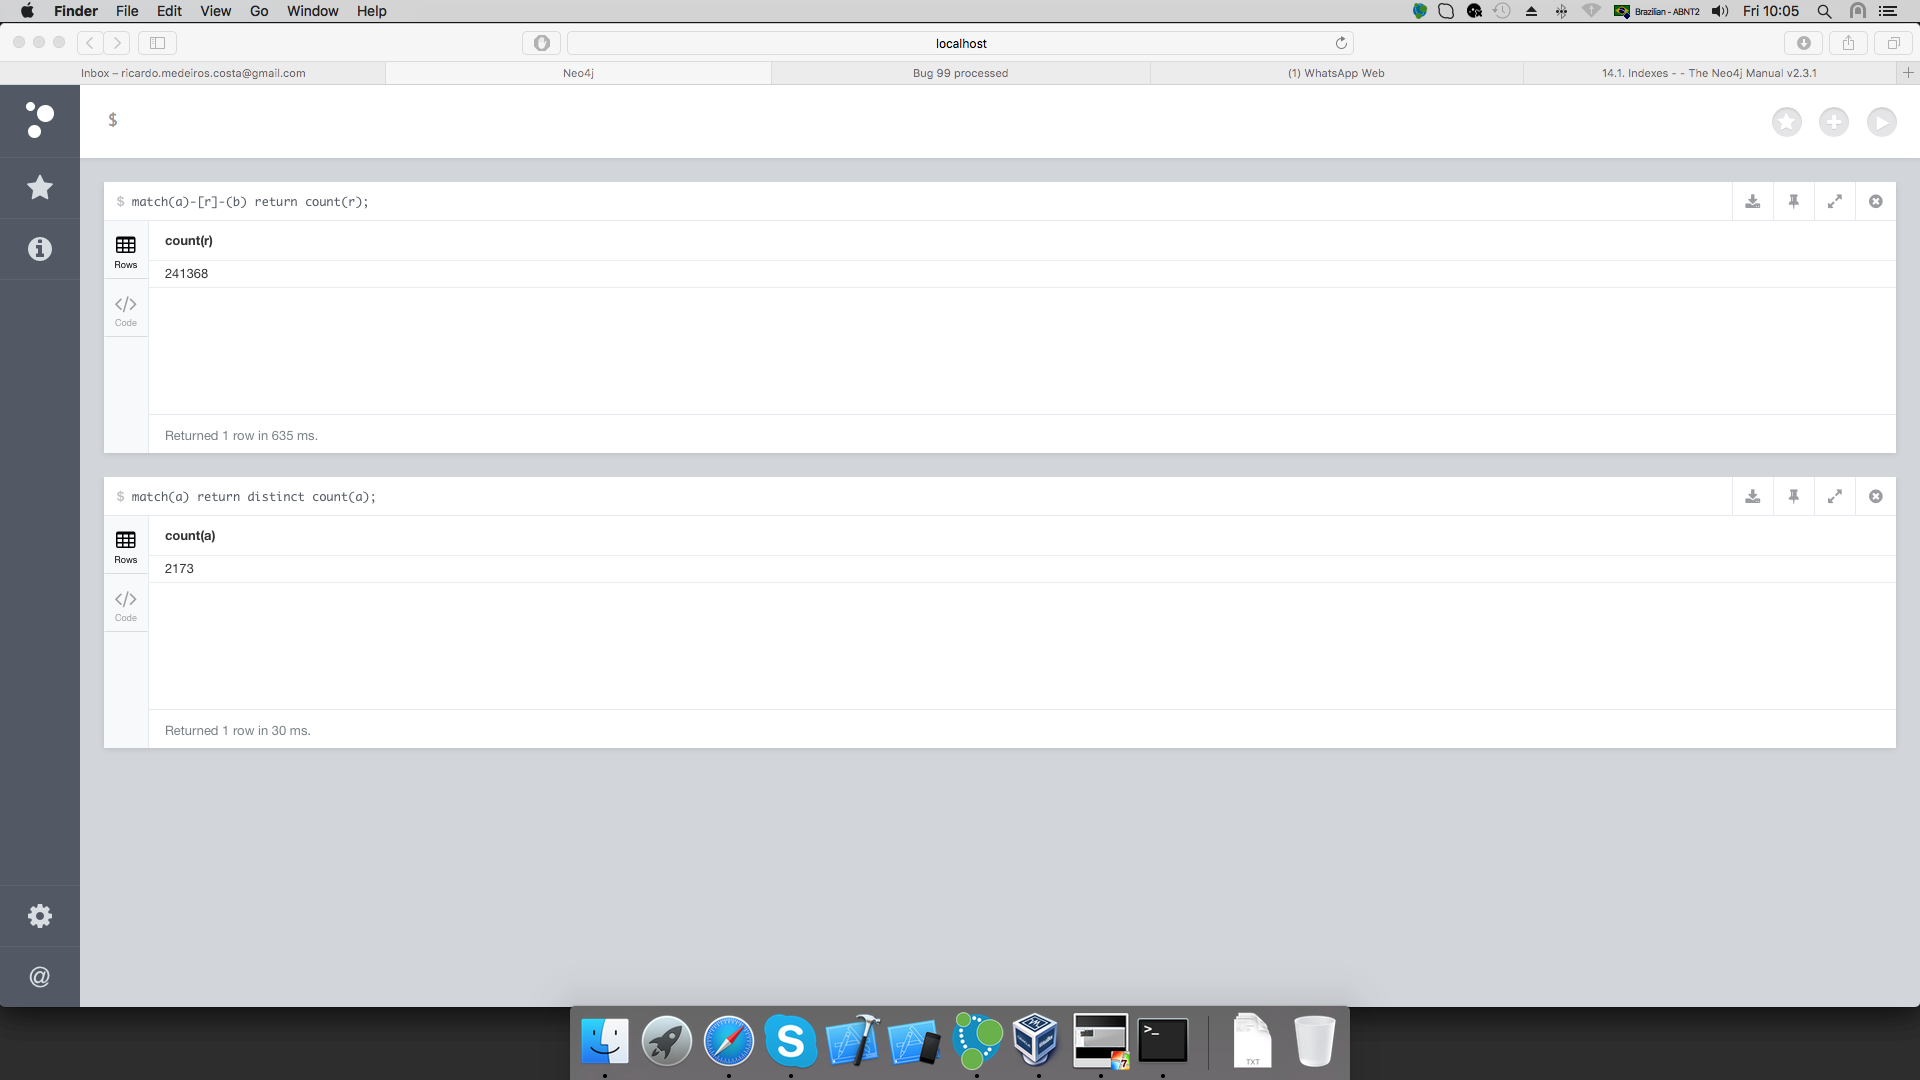
\includegraphics[width=1\textwidth]{1}
         \caption[1 - Quantidade de nós e relações]{\textbf{Quantidade de nós e relações}}
         \end{figure} 
         
    \end{description}
  \item Dados um número inteiro posititivo n, imprimir os n primeiros naturais ímpares.
    \begin{description}
      \item[Análise do Problema:] O exercício pede que após o usuário informar um número natural, seja impresso na tela os n primeiros naturais ímpares. É possível resolver isso solicitando a entrada pelo usuário, validá-la (verificar se é um natural. Ou seja, um número inteiro positivo), obter todos os números ímpares até o determinado número (verificando se o resto da divisão do número em questão é diferente a zero) e mostrar esses números para o usuário.

      \item[Algoritmo:]
         \begin{figure}[H]
         \centering
         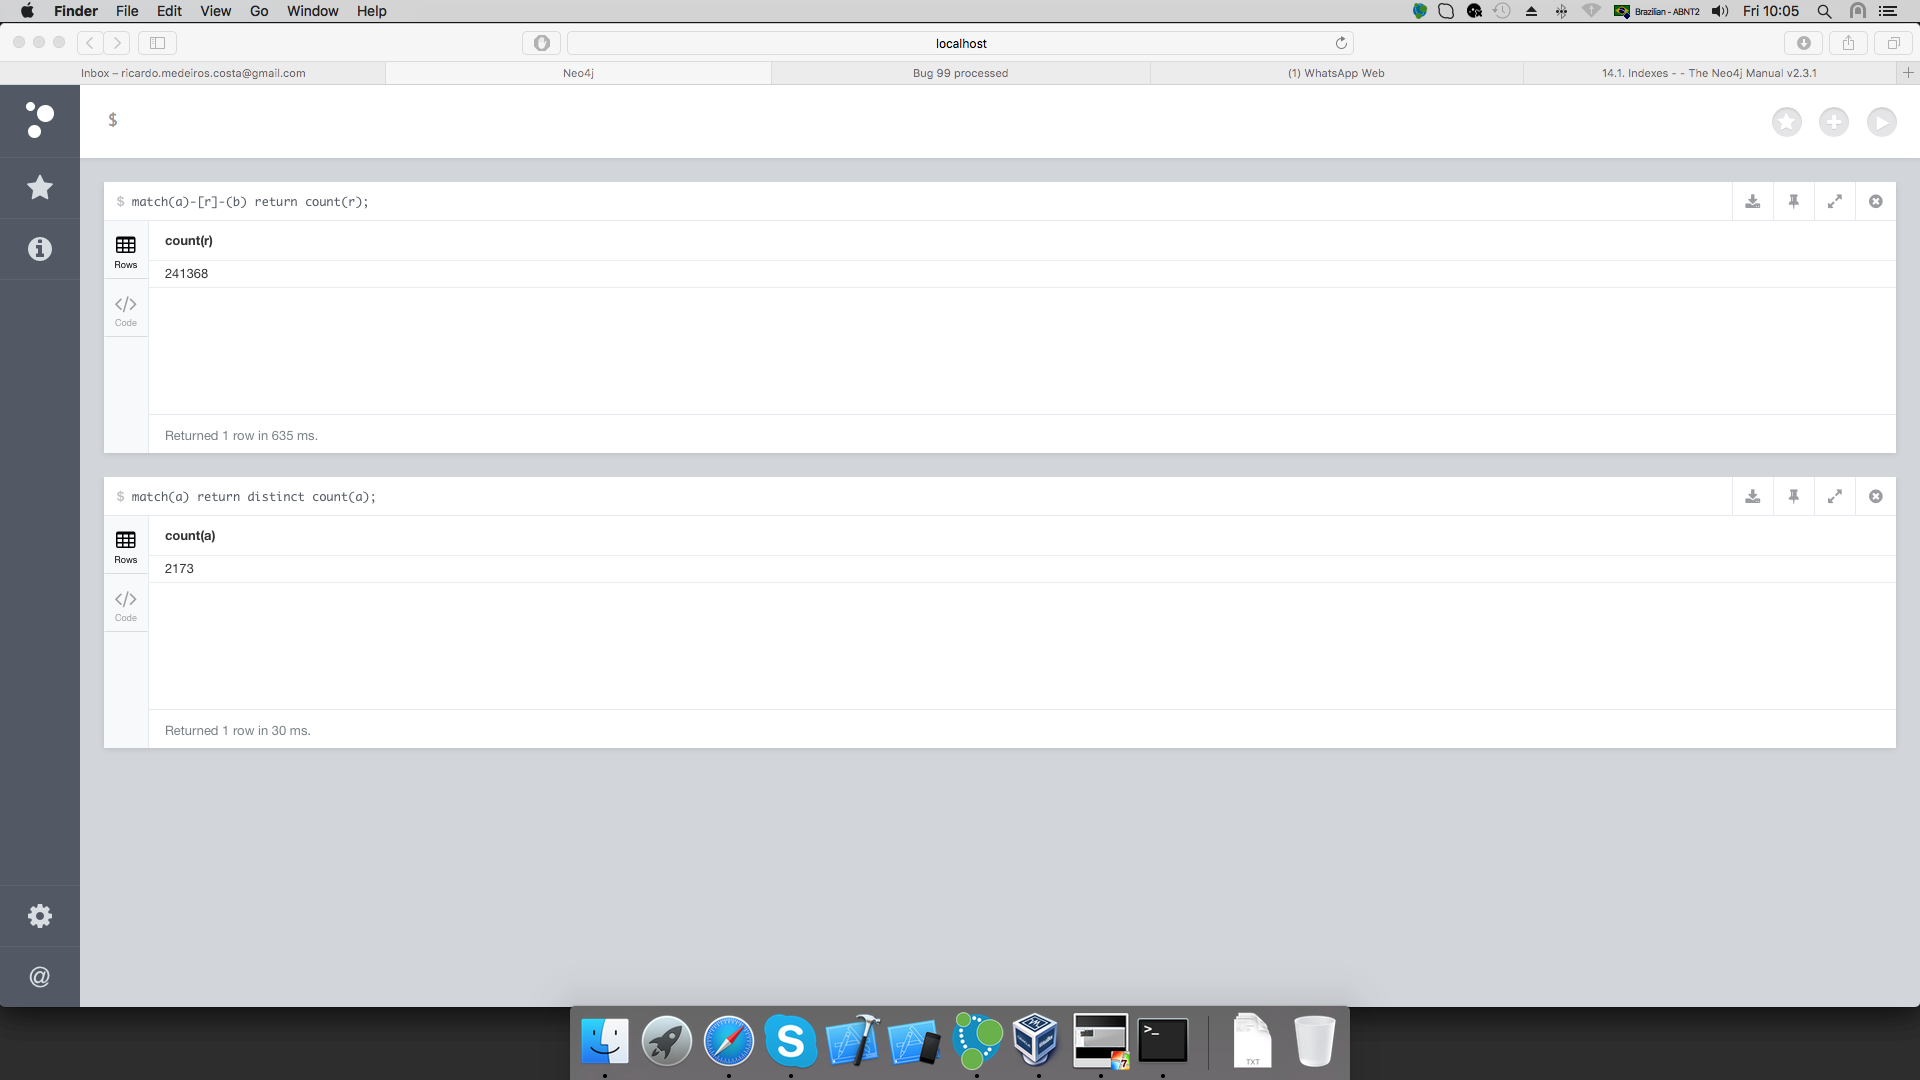
\includegraphics[width=1\textwidth]{1}
         \caption[1 - Quantidade de nós e relações]{\textbf{Quantidade de nós e relações}}
         \end{figure} 
        
       \item[Fluxograma:]
         \begin{figure}[H]
         \centering
         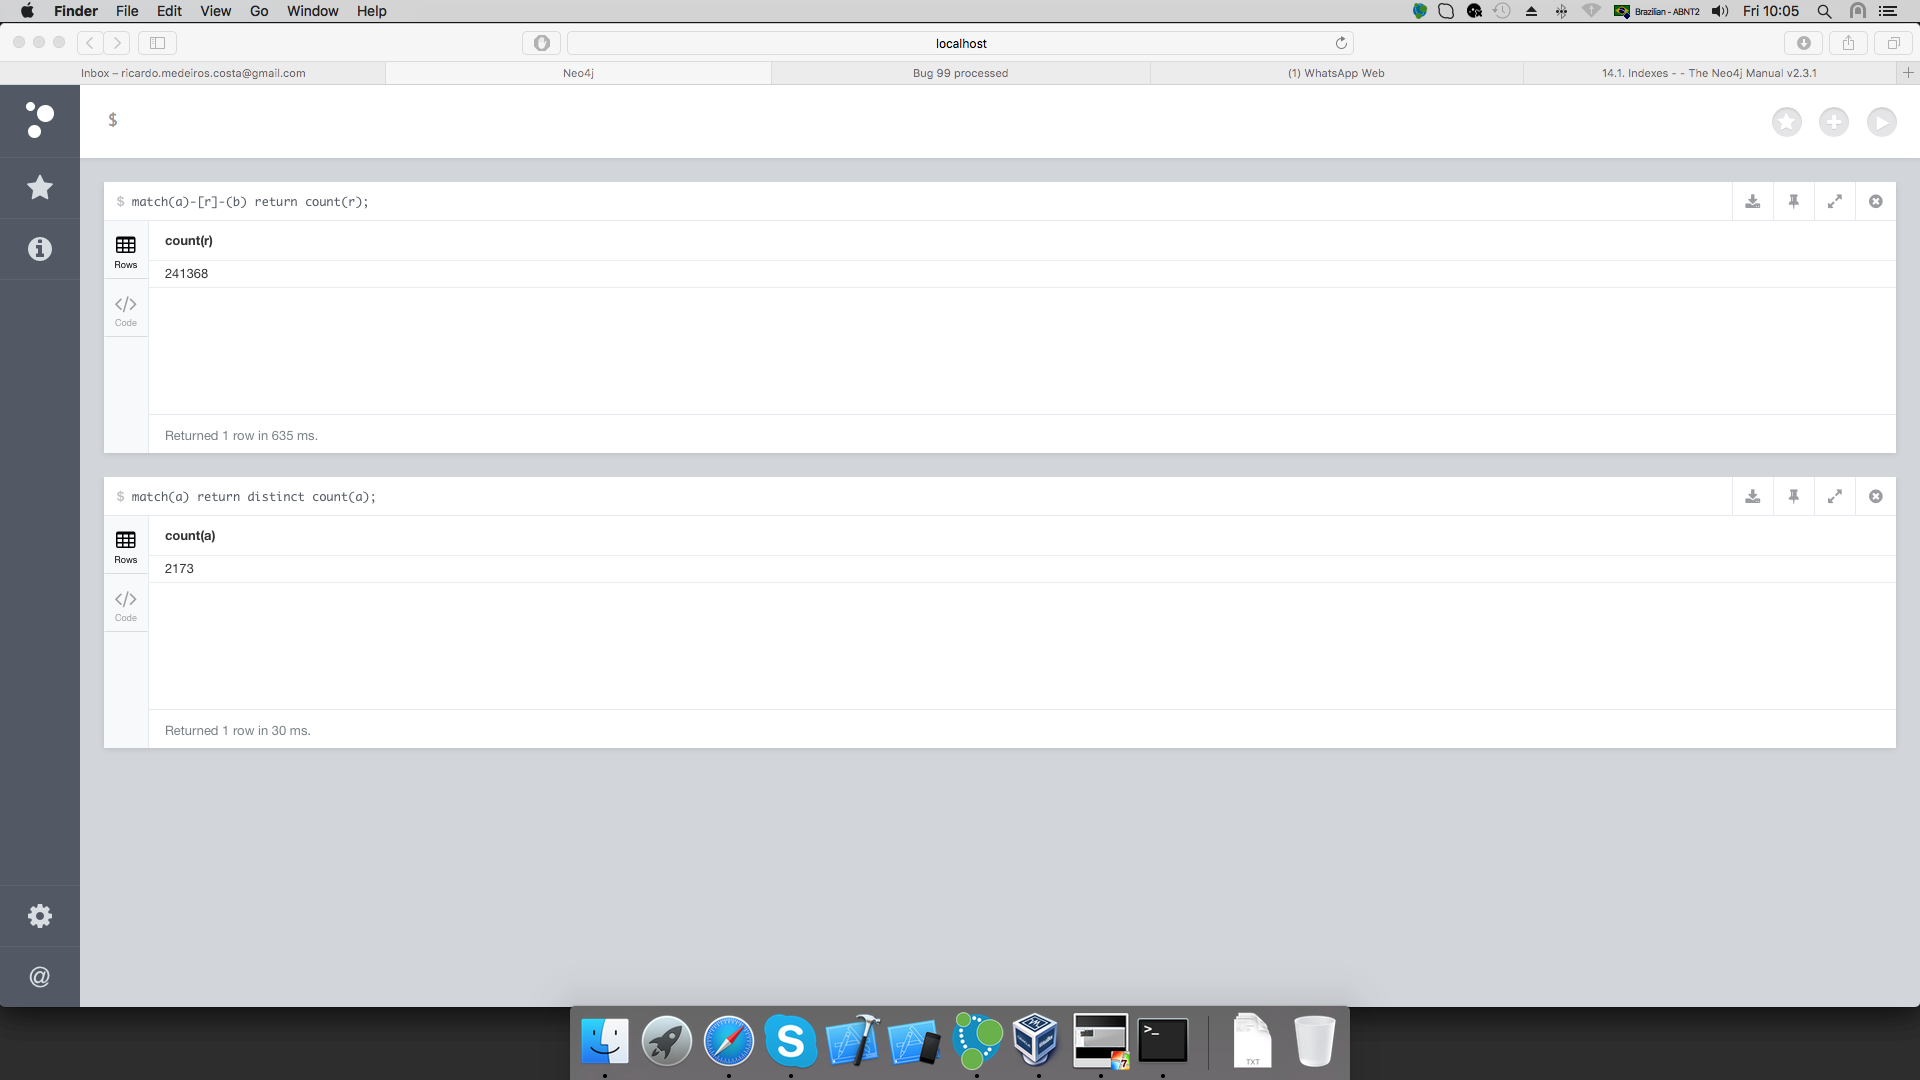
\includegraphics[width=1\textwidth]{1}
         \caption[1 - Quantidade de nós e relações]{\textbf{Quantidade de nós e relações}}
         \end{figure} 
         
       \item[Teste de mesa:]
         \begin{figure}[H]
         \centering
         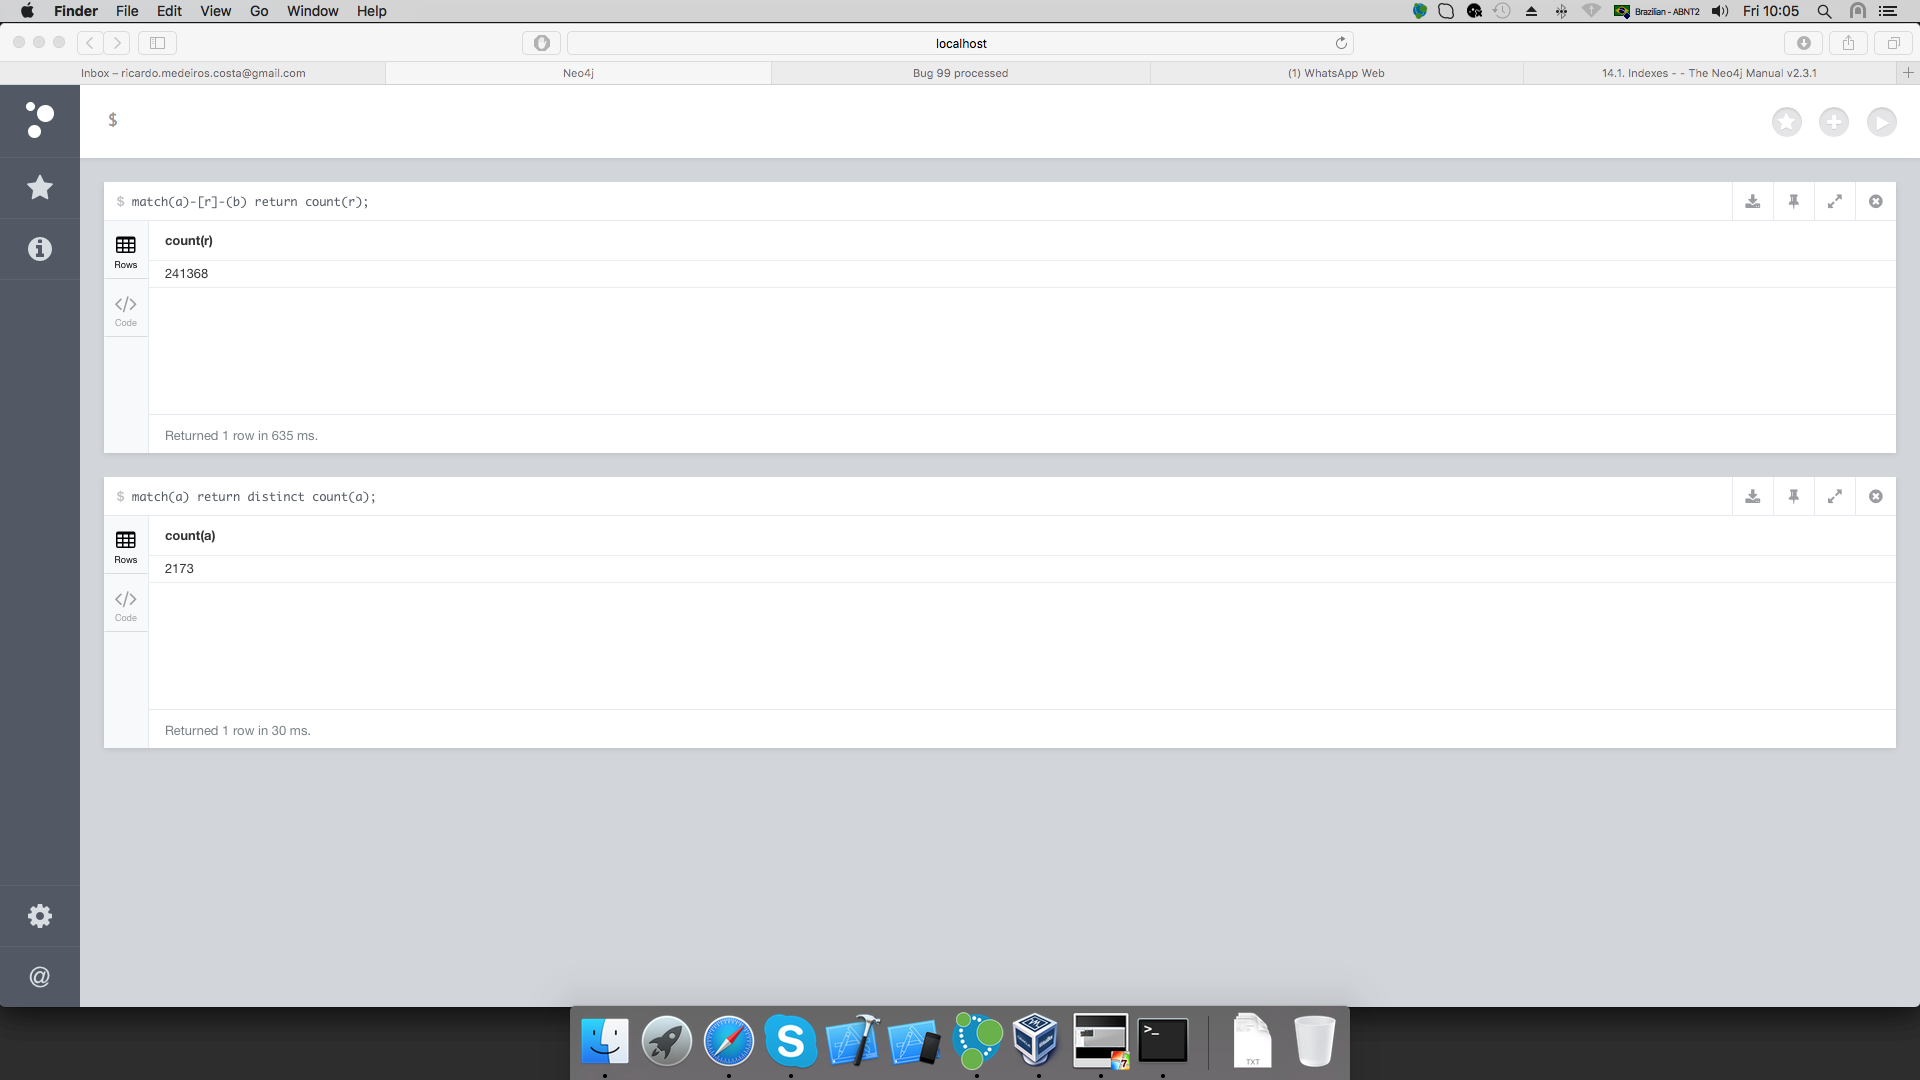
\includegraphics[width=1\textwidth]{1}
         \caption[1 - Quantidade de nós e relações]{\textbf{Quantidade de nós e relações}}
         \end{figure} 
         
    \end{description}
  \item Dado um número real na base binária, transformá-lo para base decimal.
    \begin{description}
      \item[Análise do Problema:] O exercício pede que converta um número natural de base binária para um número de base decimal. Uma alternativa é validar a entrada do usuário se realmente é um número natural de base binária (verificando se os dígitos são 0 ou 1 e se é um número natural), converter o número (realizando o somatório de cada termo multiplicado por 2 elevado a n-i, cujo n é a quantidade de dígitos e i é a posição atual) e informando o resultado para o usuário.

      \item[Algoritmo:]
         \begin{figure}[H]
         \centering
         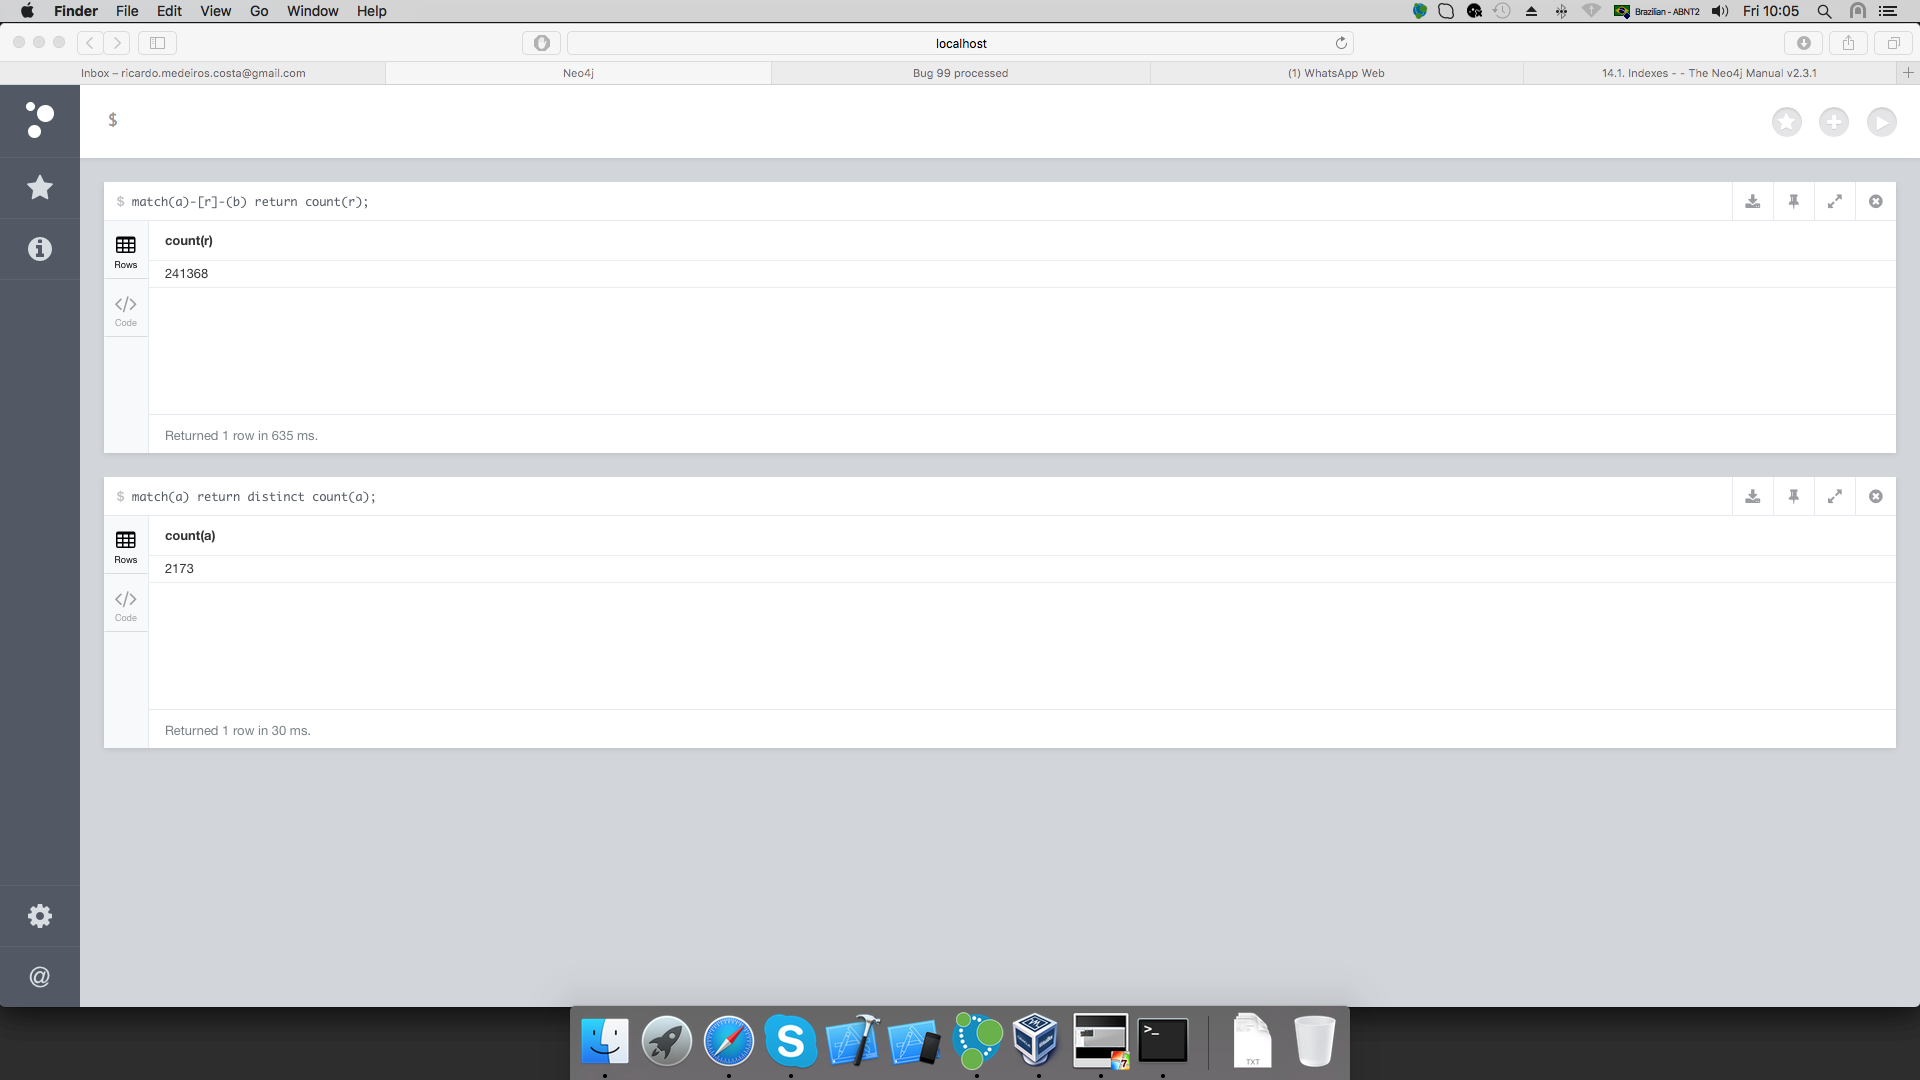
\includegraphics[width=1\textwidth]{1}
         \caption[1 - Quantidade de nós e relações]{\textbf{Quantidade de nós e relações}}
         \end{figure} 
        
       \item[Fluxograma:]
         \begin{figure}[H]
         \centering
         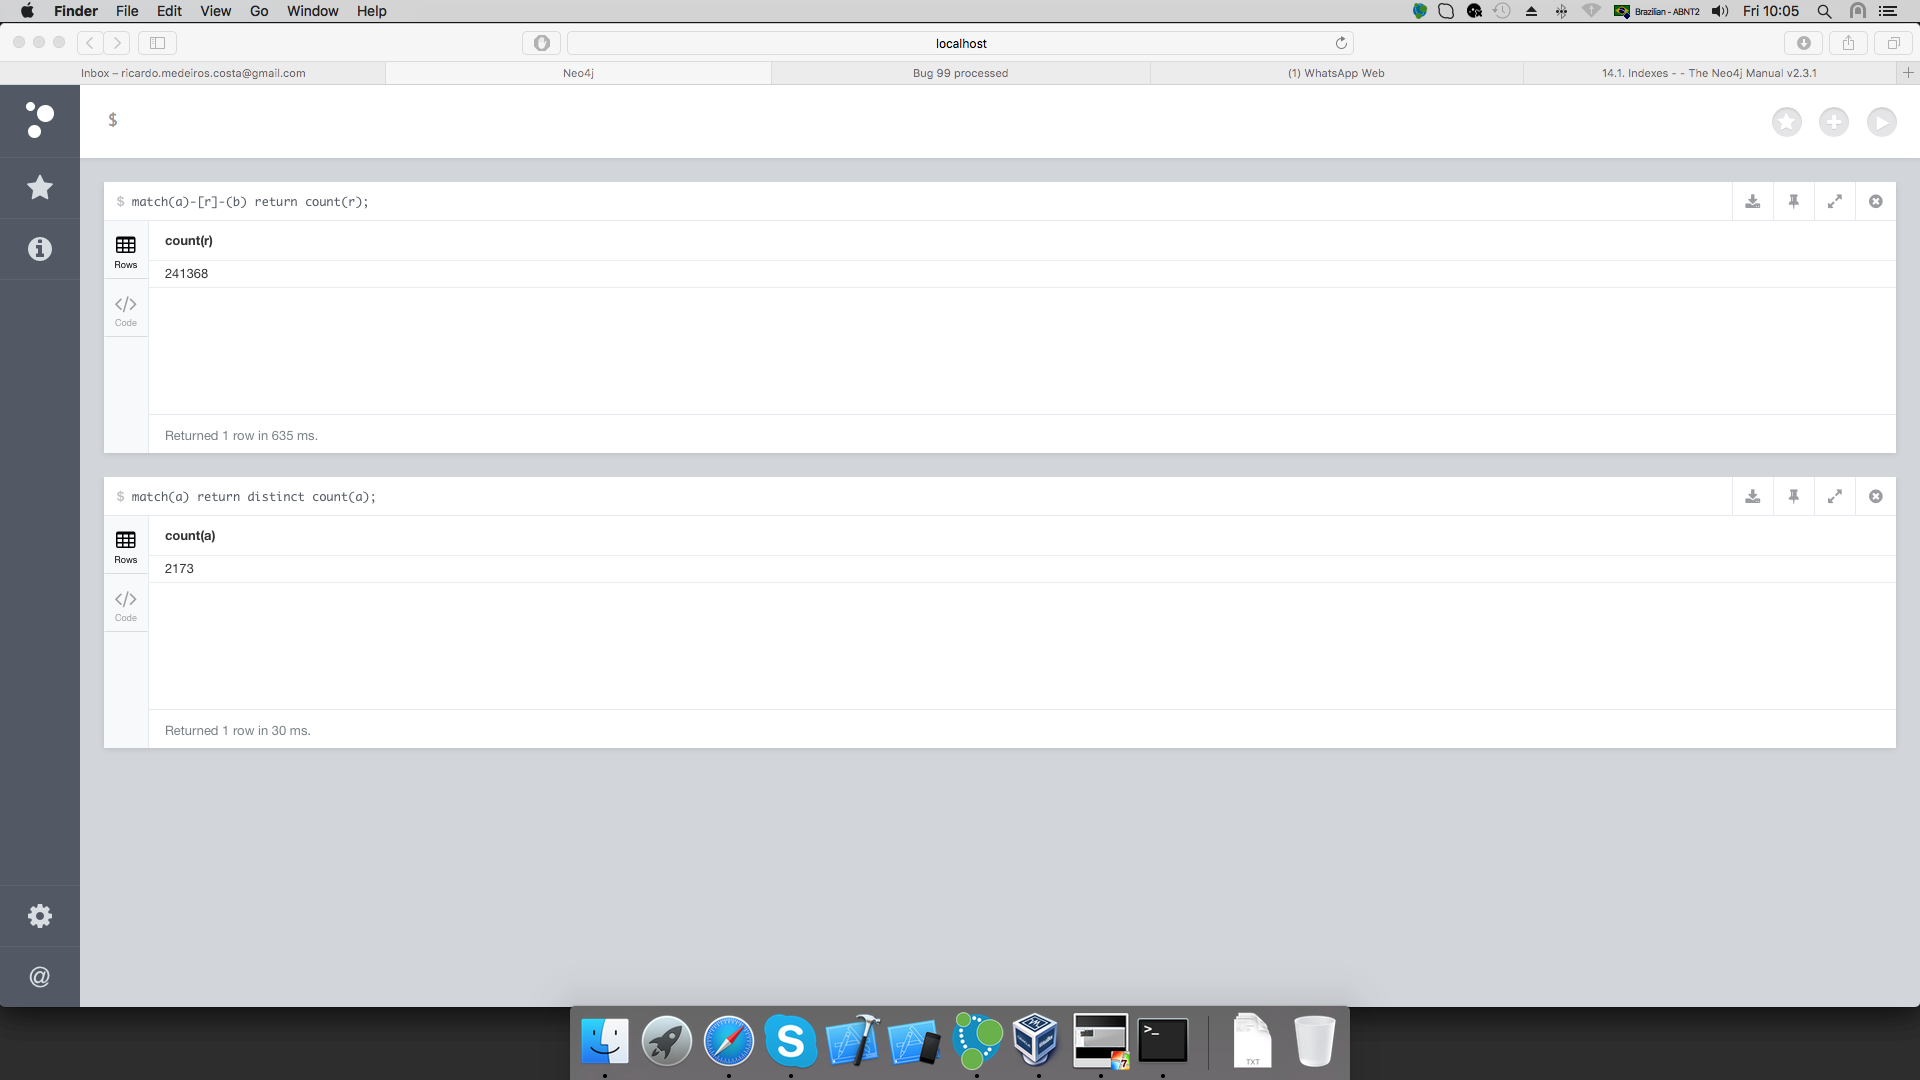
\includegraphics[width=1\textwidth]{1}
         \caption[1 - Quantidade de nós e relações]{\textbf{Quantidade de nós e relações}}
         \end{figure} 
         
       \item[Teste de mesa:]
         \begin{figure}[H]
         \centering
         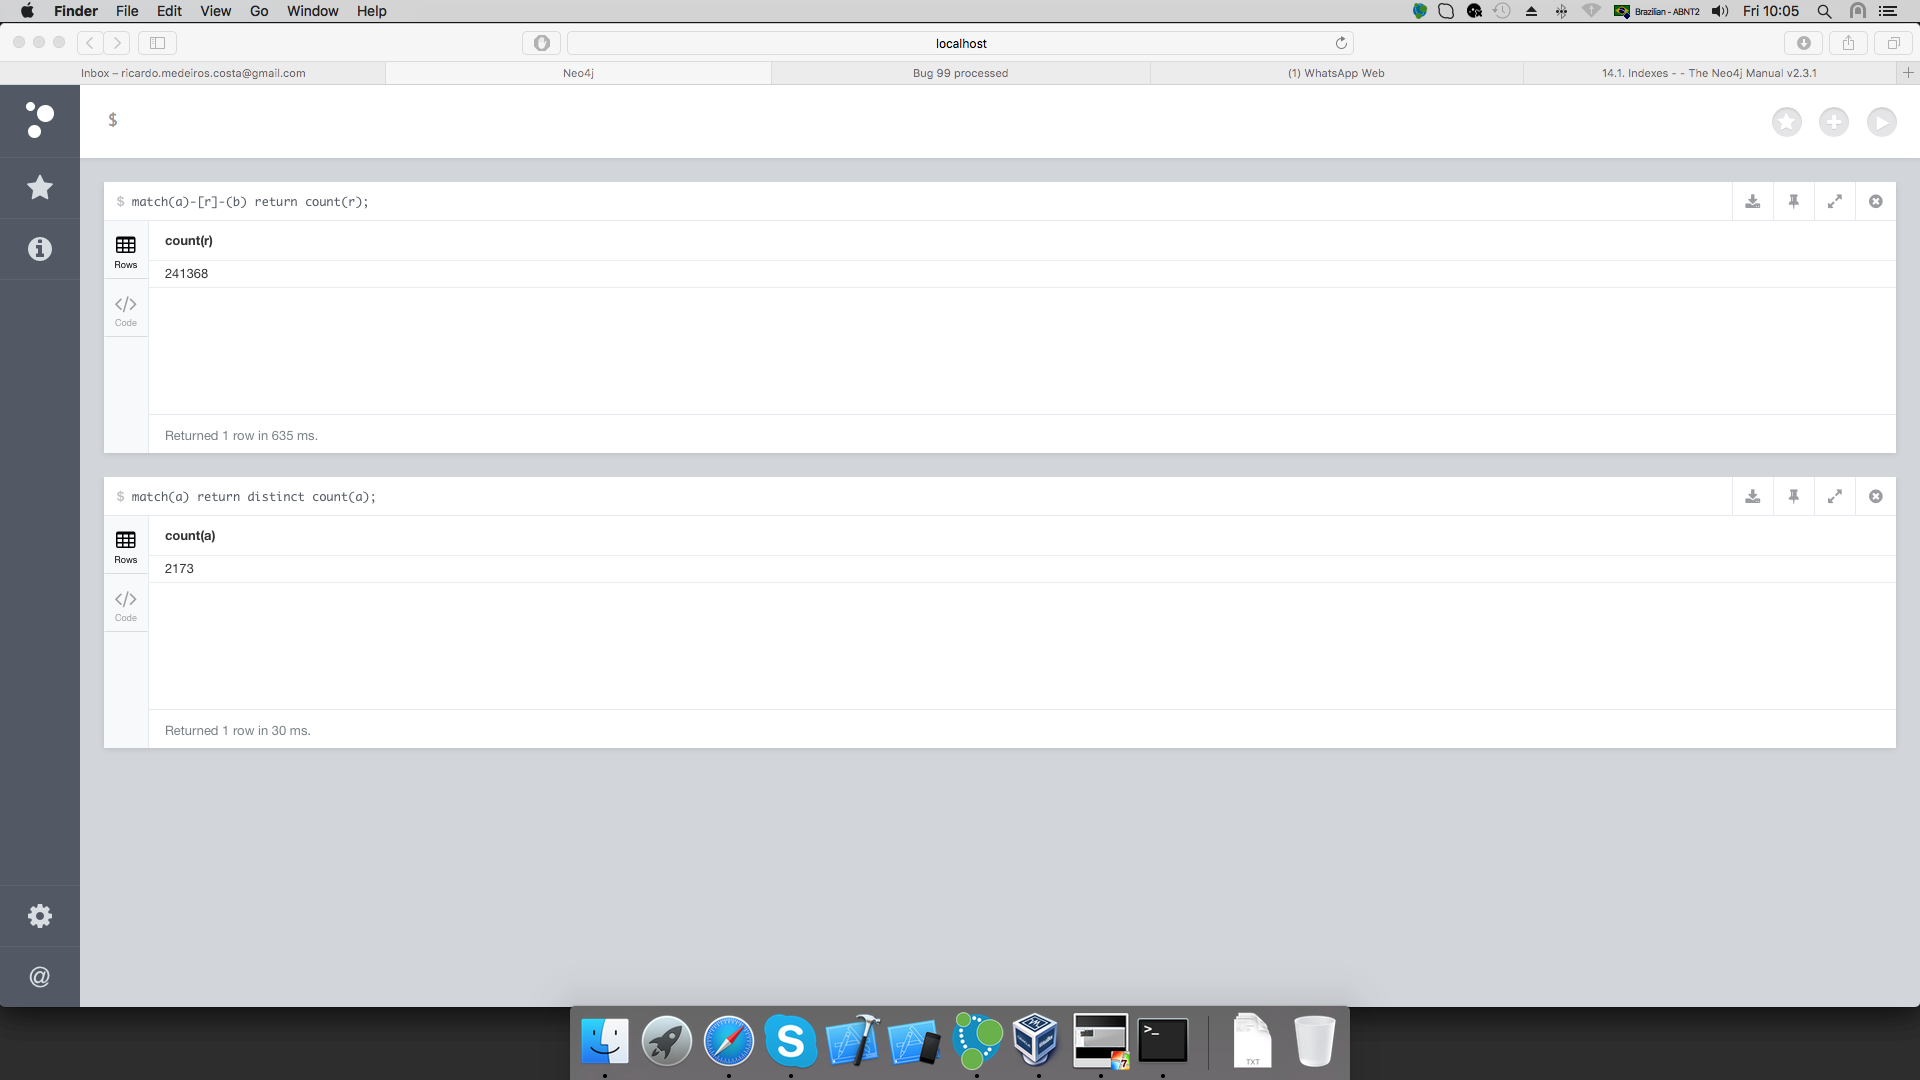
\includegraphics[width=1\textwidth]{1}
         \caption[1 - Quantidade de nós e relações]{\textbf{Quantidade de nós e relações}}
         \end{figure} 
         
    \end{description}
      \item Dado um número natural > 10, verificar se n é palíndromo.
    \begin{description}
      \item[Análise do Problema:] O exercício pede para verificar se uma entrada informada por um usuário é um número palíndromo. Por definição, um número palíndromo é igual ao seu reverso. Então para solucionar esse problema é capturada a entrada pelo usuário, verifica-se se o número natural é maior que 11 (uma restrição do enunciado), obtém seu reverso e realiza-se a comparação do número informado com o seu reverso. Se forem iguais, o número é palíndromo; se não forem, não é.

      \item[Algoritmo:]
         \begin{figure}[H]
         \centering
         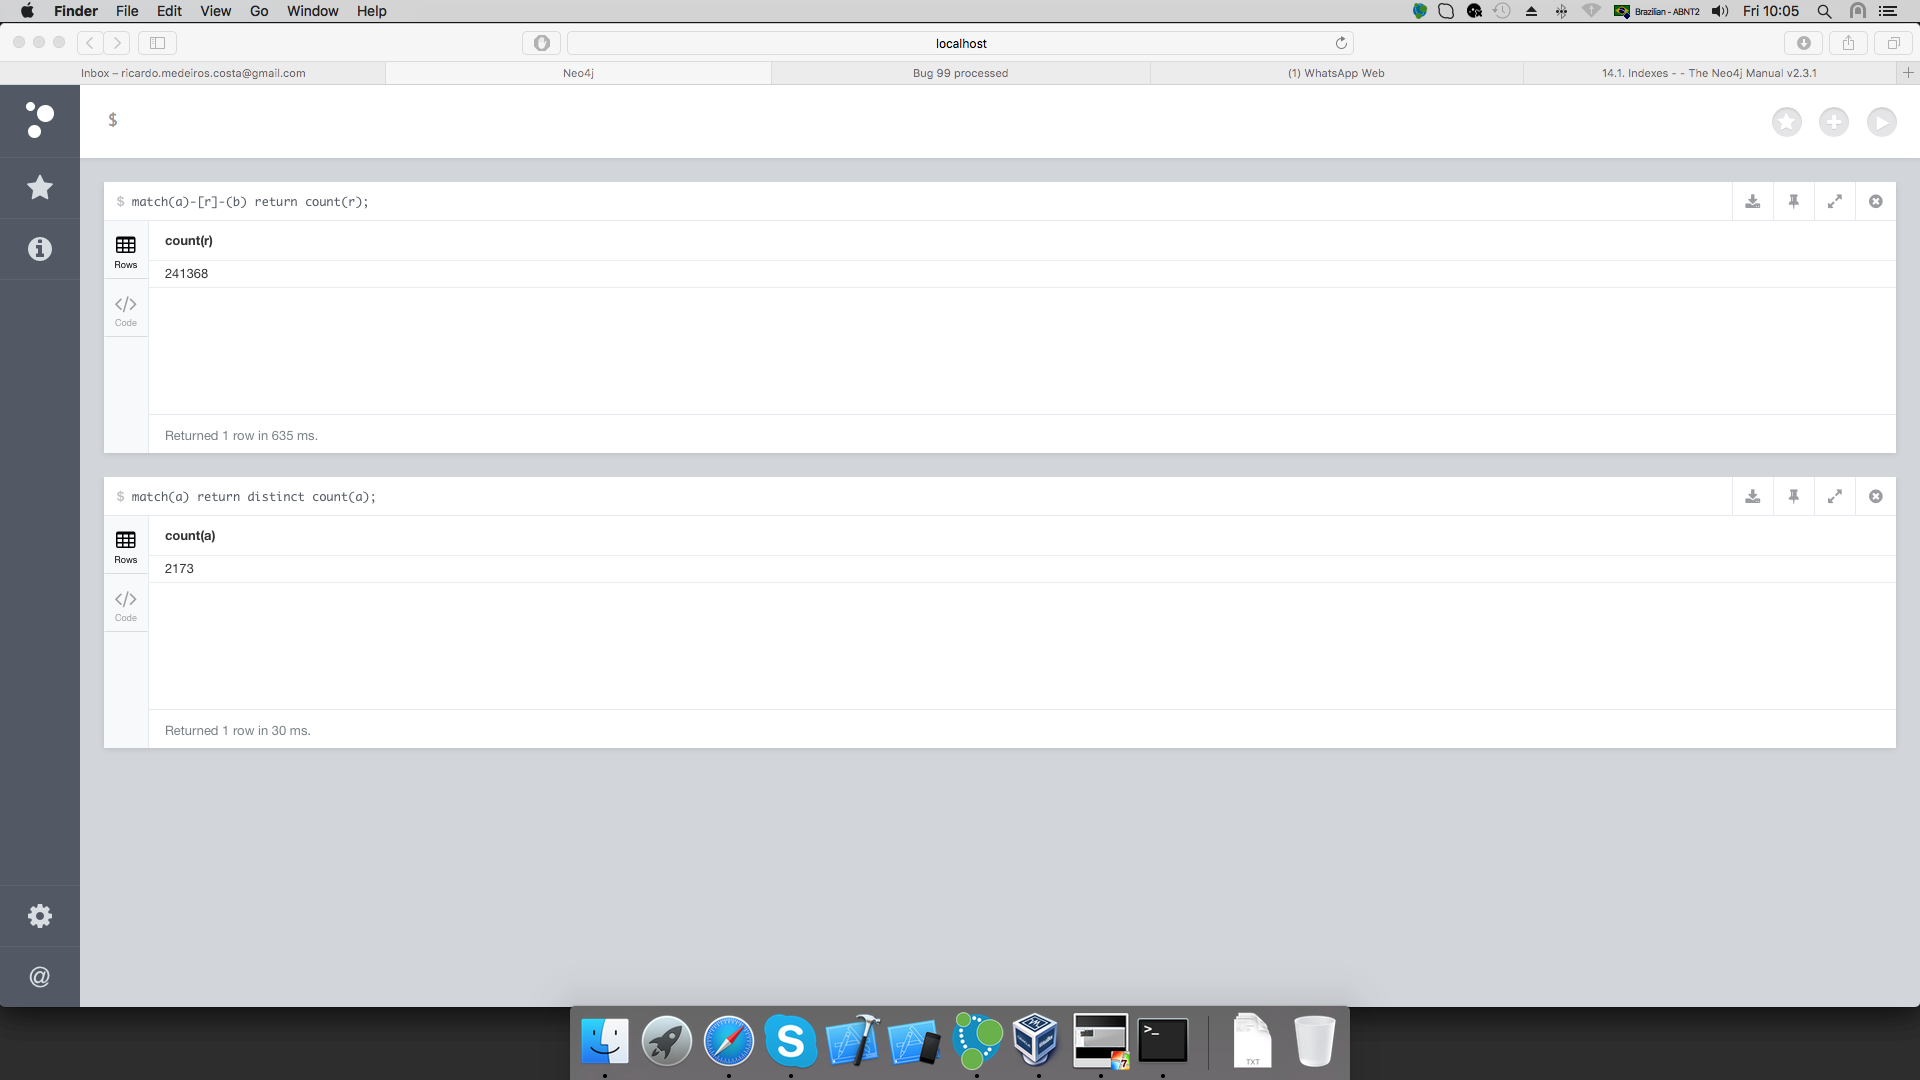
\includegraphics[width=1\textwidth]{1}
         \caption[1 - Quantidade de nós e relações]{\textbf{Quantidade de nós e relações}}
         \end{figure} 
        
       \item[Fluxograma:]
         \begin{figure}[H]
         \centering
         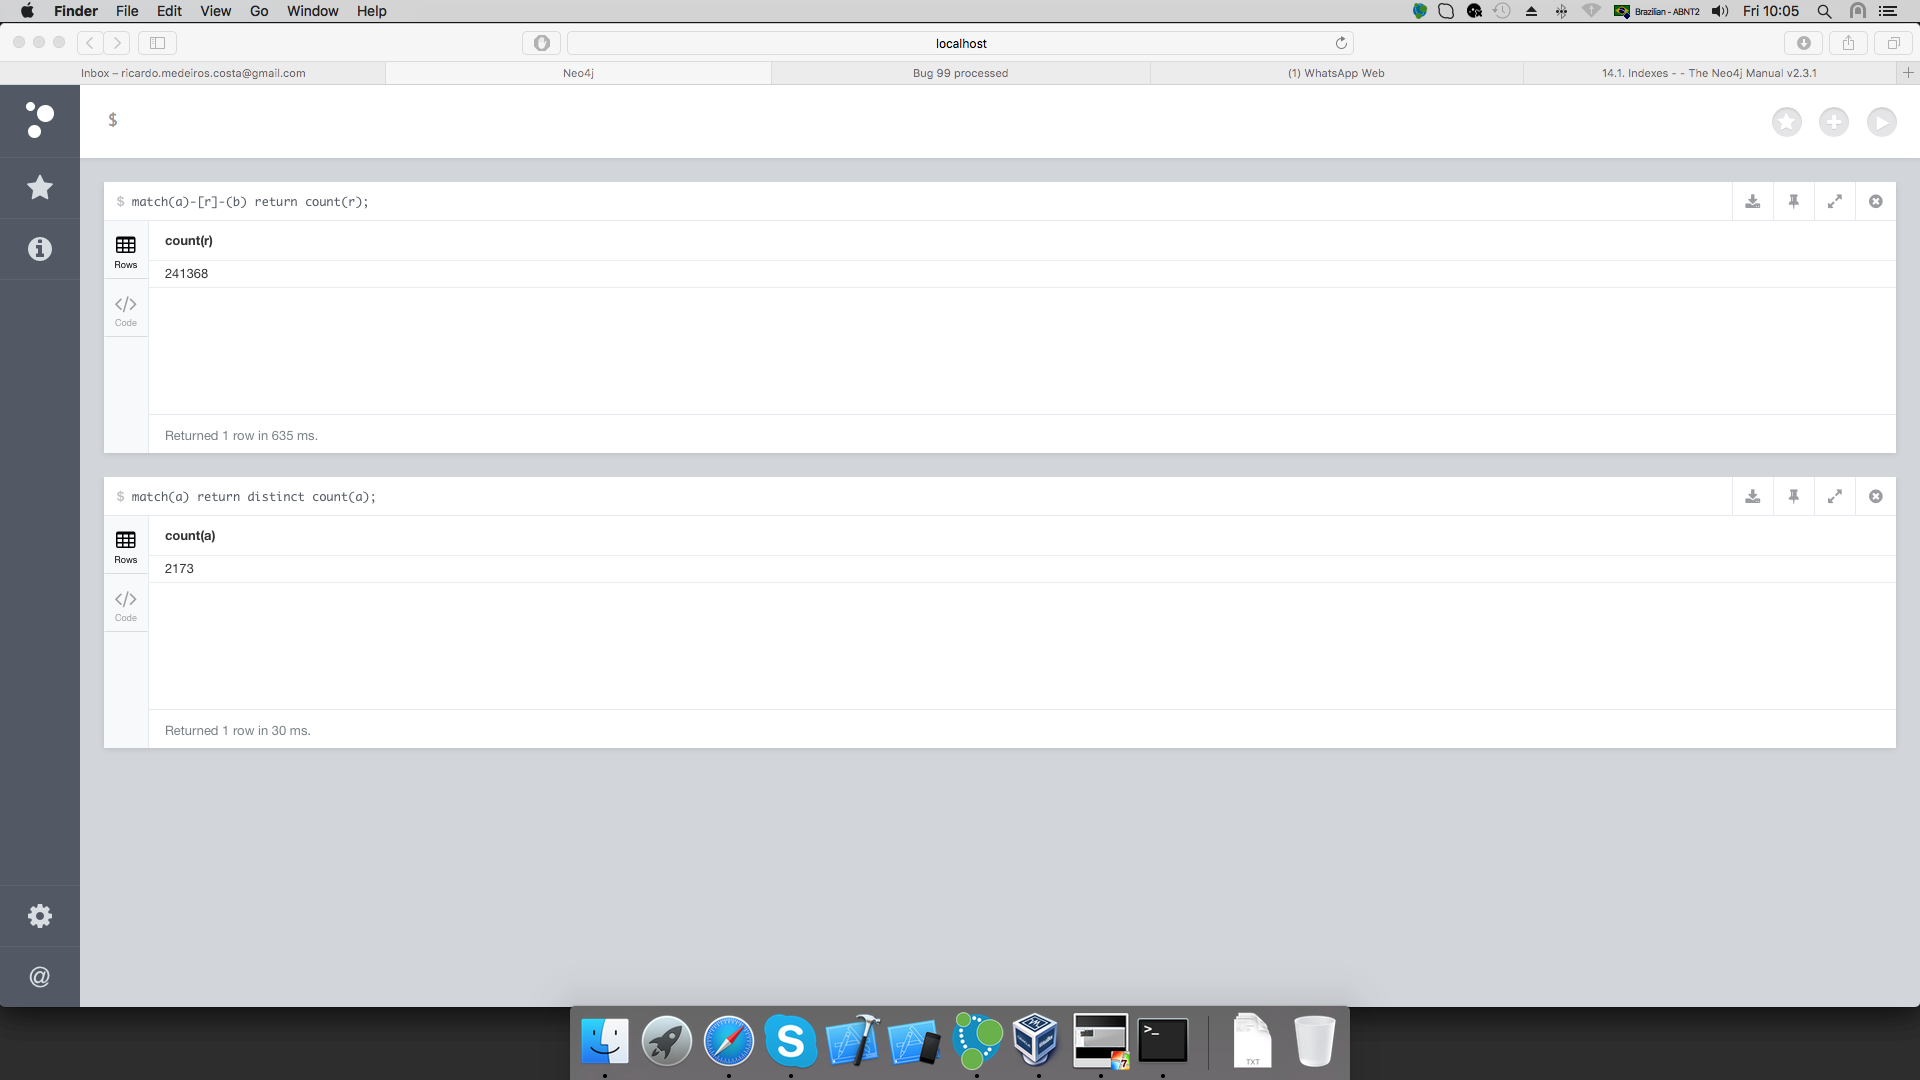
\includegraphics[width=1\textwidth]{1}
         \caption[1 - Quantidade de nós e relações]{\textbf{Quantidade de nós e relações}}
         \end{figure} 
         
       \item[Teste de mesa:]
         \begin{figure}[H]
         \centering
         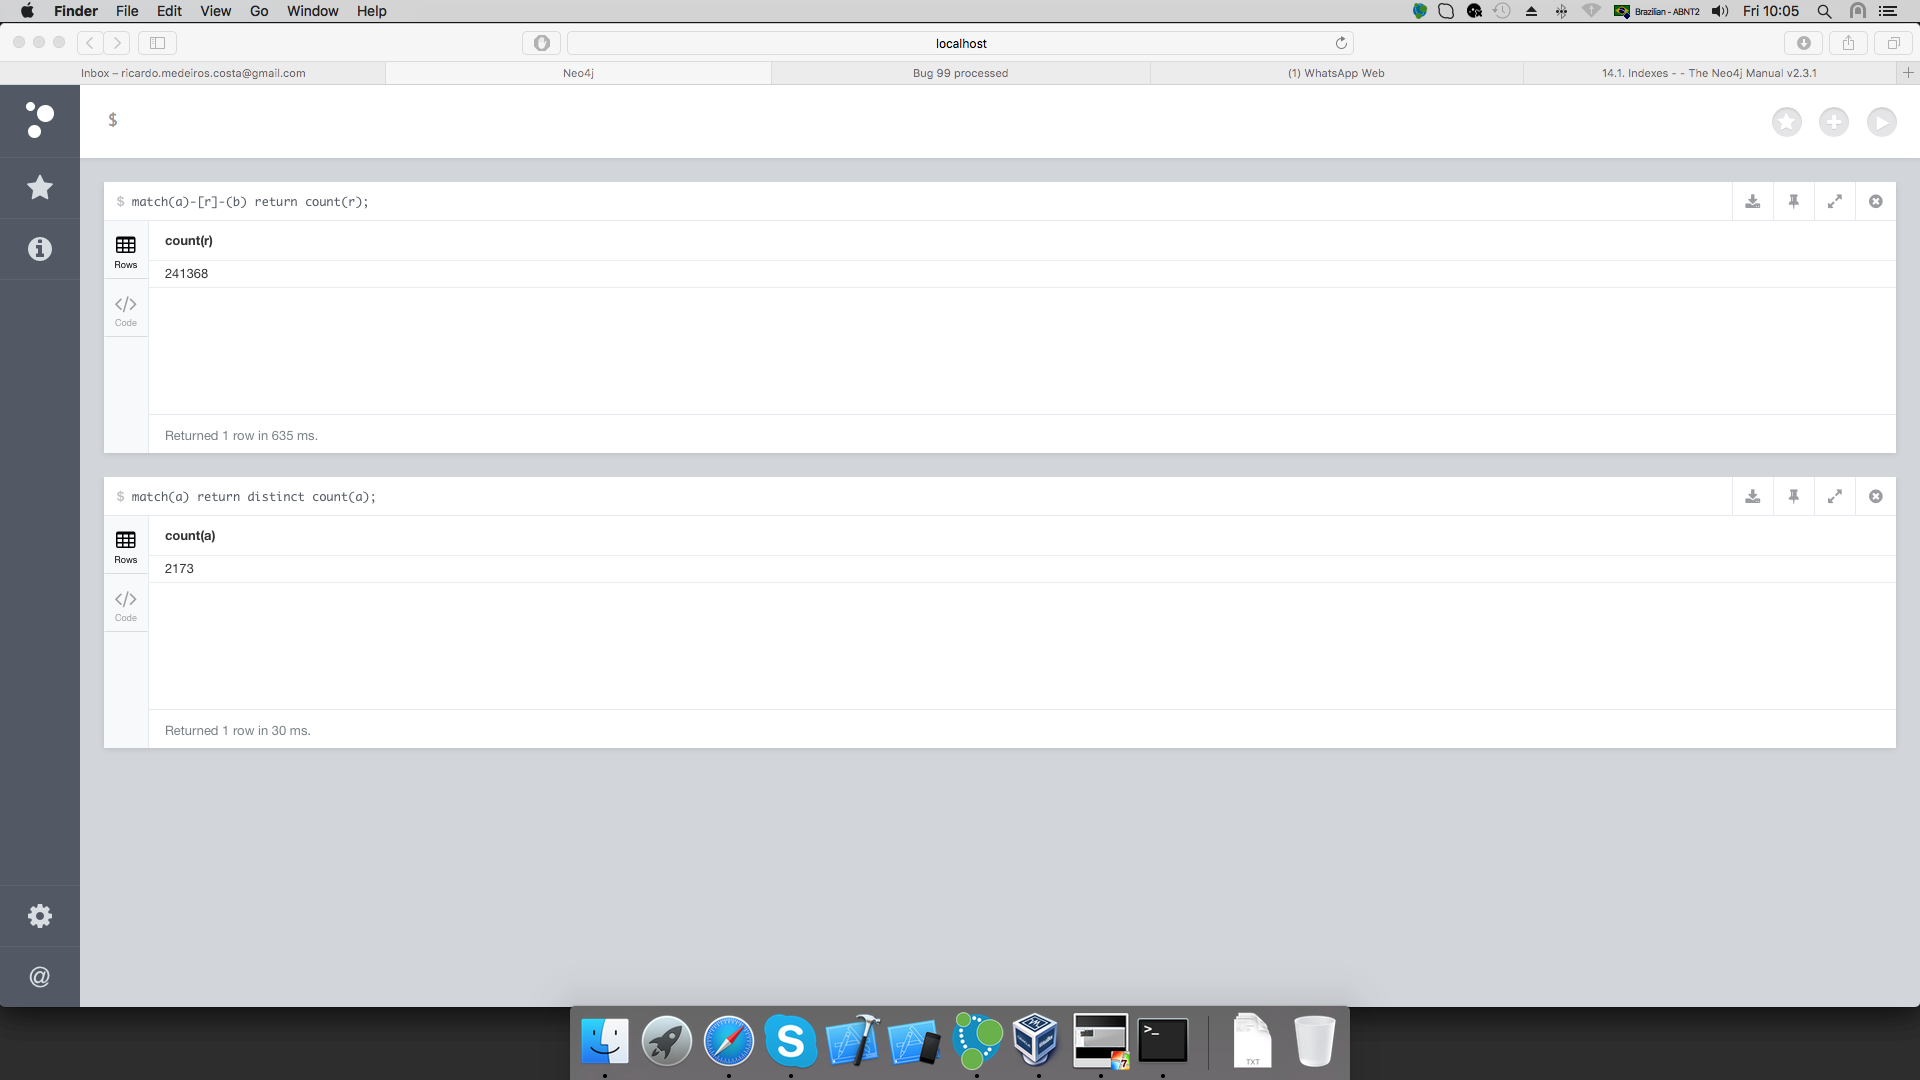
\includegraphics[width=1\textwidth]{1}
         \caption[1 - Quantidade de nós e relações]{\textbf{Quantidade de nós e relações}}
         \end{figure} 
         
    \end{description}
\end{enumerate}

\end{enumerate}
\end{enumerate}


\end{document}
